\documentclass[11pt,fleqn]{article}
\usepackage[margin=1in,top=1in,bottom=1in]{geometry}
\usepackage{tikz}
\usepackage{mathtools}
\usepackage{longtable}
\usepackage{enumitem}
\usepackage{hyperref}
%\usepackage[dvips]{graphics}
%\usepackage[table]{xcolor}
%\usepackage{amssymb}
\usepackage{float}
%\usepackage{subfig}
\usepackage{booktabs}
\usepackage{subcaption}

\usepackage[normalem]{ulem}

\usepackage{multicol}
\usepackage{txfonts}
\usepackage{amsfonts}
\usepackage{natbib}
\usepackage{gb4e}
\usepackage[all]{xy}
\usepackage{rotating}
\usepackage{tipa}
\usepackage{multirow}
\usepackage{authblk}
\usepackage{url}
\usepackage{pdflscape}
\usepackage{rotating}
\usepackage{adjustbox}
\usepackage{array}


\def\bad{{\leavevmode\llap{*}}}
\def\marginal{{\leavevmode\llap{?}}}
\def\verymarginal{{\leavevmode\llap{??}}}
\def\swmarginal{{\leavevmode\llap{4}}}
\def\infelic{{\leavevmode\llap{\#}}}

\definecolor{airforceblue}{rgb}{0.36, 0.54, 0.66}
%\definecolor{gray}{rgb}{0.36, 0.54, 0.66}

\definecolor{Pink}{RGB}{240,0,120}
\newcommand{\red}[1]{\textcolor{Pink}{#1}}
\newcommand{\jd}[1]{\textbf{\textcolor{Pink}{[jd: #1]}}}

\newcommand{\dashrule}[1][black]{%
  \color{#1}\rule[\dimexpr.5ex-.2pt]{4pt}{.4pt}\xleaders\hbox{\rule{4pt}{0pt}\rule[\dimexpr.5ex-.2pt]{4pt}{.4pt}}\hfill\kern0pt%
}

\setlength{\parindent}{.3in}
\setlength{\parskip}{0ex}

\newcommand{\yi}{\'{\symbol{16}}}
\newcommand{\nasi}{\~{\symbol{16}}}
\newcommand{\hina}{h\nasi na}
\newcommand{\ina}{\nasi na}

\newcommand{\foc}{$_{\mbox{\small F}}$}

\hyphenation{par-ti-ci-pa-tion}

\setlength{\bibhang}{0.5in}
\setlength{\bibsep}{0mm}
\bibpunct[:]{(}{)}{,}{a}{}{,}

\newcommand{\6}{\mbox{$[\hspace*{-.6mm}[$}} 
\newcommand{\9}{\mbox{$]\hspace*{-.6mm}]$}}
\newcommand{\sem}[2]{\6#1\9$^{#2}$}
\renewcommand{\ni}{\~{\i}}

\newcommand{\citepos}[1]{\citeauthor{#1}'s \citeyear{#1}}
\newcommand{\citeposs}[1]{\citeauthor{#1}'s}
\newcommand{\citetpos}[1]{\citeauthor{#1}'s (\citeyear{#1})}

\newcolumntype{R}[2]{%
    >{\adjustbox{angle=#1,lap=\width-(#2)}\bgroup}%
    l%
    <{\egroup}%
}
\newcommand*\rot{\multicolumn{1}{R{90}{0em}}}% no optional argument here, please!


\title{Does at-issueness predict projection? Further investigations of the Gradient Projection Principle}

%\thanks{For helpful comments on the research presented here, we thank David Beaver, Cleo Condoravdi, Kai von Fintel, Lauri Karttunen, Mandy Simons, Greg Scontras, the anonymous reviewers for {\em Semantics and Linguistic Theory} 2018, as well as the audiences at the MIT Linguistics colloquium, the 2018 Annual Meeting of XPRAG.de and at the University of T\"ubingen. We gratefully acknowledge financial support for this research from {\em National Science Foundation} grant BCS-1452674 (JT) and the Targeted Investment for Excellence Initiative at The Ohio State University (JT). IGOR Tuebingen, SALT TALK}}

\author{Author(s)}

%\author[$\circ$]{Judith Tonhauser}
%\author[$\bullet$]{Judith Degen}
%\affil[$\circ$]{The Ohio State University / University of Stuttgart}
%\affil[$\bullet$]{Stanford University}
%
%\renewcommand\Authands{ and }

\newcommand{\jt}[1]{\textbf{\color{blue}JT: #1}}

\begin{document}

%\tableofcontents
%\newpage

\maketitle

\vspace*{-1cm}

\begin{abstract}

\citealt{tbd-variability} hypothesized that at-issueness is one factor that modulates the projection of content (see also \citealt{brst-salt10,brst-ar}). Specifically, according to their Gradient Projection Principle, if content $C$ is expressed by a constituent embedded under an entailment-canceling operator, then $C$ projects to the extent that it is not at-issue. Their work provided evidence for the GPP from xx contents that had been described as projective in the literature, at-issueness was measured in two different ways, only one consistently brought evidence in support (question, asking whether, are you sure? mixed results 2b). This paper provides further investigate the GPP by investigating a) more varied items, b) with more types of embedding, and c) other measures of at-issueness. These experiments provide additional support for the GPP, and they also show: comparison of projection across entailment-canceling operators, comparison of at-issueness diagnostics. Suggests that the diagnostics may not all measure the same (\citealt{snider2017}).

\end{abstract}

\newpage

\tableofcontents

\newpage
		
\section{Introduction}\label{s1}

Prijection comparison hasn't been done, except in CommitmentBank paper (right?, perhaps A'dam colloquium presentation?).

\begin{exe}
\ex Context: A and B live near a dog that regularly barks for extended periods of time. It is barking right now. A says:  \\ Ugh. The damn dog is barking again.
\end{exe}

Contents:

\begin{itemize}
\item there is a unique salient dog (backgrounded, ps)
\item the dog has barked before (backgrounded, ps)
\item the speaker is annoyed at the dog/barking (new, could be what the speaker wants to contribute)
\item the dog is barking (``at-issue'', ordinary entailment)
\end{itemize}

First dimension: Role in discourse context: some anchor to context, some convey relevant backgrounded information, some are what the speaker wants to communicate.

Second dimension: Compositional semantics: some interact, some don't.

Third dimension: Role in subsequent discourse: some are what carries the conversation on, some do not.


One of the contents is privileged in that it is the content that is put up for negotiation. It is often new information, though not necessarily. It is what is ``linguistically relevant'': it interacts with operators and is accessible for anaphoric reference.


\begin{exe}
\ex\label{gpp} {\bf Gradient Projection Principle} \hfill (\citealt[400]{tbd-variability}) \\ If content $C$ is expressed by a constituent embedded under an entailment-canceling operator, then $C$ projects to the extent that it is not at-issue.
\end{exe}

We already know that the GPP is stated too strongly: prior influences projection (\citealt{degen-tonhauser-openmind}) {\bf independently of at-issueness (unpublished)}. At-issueness is one factor among many.


\begin{exe}
\ex\label{rqs} {\bf Main research question} \\
Are not-at-issueness and projection positively correlated, as predicted by the Gradient Projection Principle?
\end{exe}

\begin{exe}
\ex\label{rqs} {\bf Ancillary research questions}
\begin{xlist}

\ex Is the at-issueness of contents embedded under different entailment-canceling operators positively correlated?

\ex Is the at-issueness of contents positively correlated under different measures of at-issueness?

\ex Compare projection under different entailment-cancelling operators

\ex Do commonly used at-issueness diagnostics work for content embedded under entailment-cancelling operators?

\end{xlist}
\end{exe}


Previous investigations of/claims about the relationship between projection and at-issueness:

\begin{itemize}

\item \citealt{brst-salt10,brst-ar}

\item \citealt{xue-onea11}

\item \citealt{tbd-variability}

\item \citealt{koev2018}

\end{itemize}

Limited how? (only presuppositions + CCs of factive predicates: \citealt{degen-tonhauser-factive} / few measures of at-issueness / some supporting results, some not / some embedded, other matrix clause)

\begin{exe}
\ex\label{pred} 20 clause-embedding predicates 

\begin{xlist}

\ex canonically factive: {\em be annoyed, discover, know, reveal, see}

\ex nonfactive:

\begin{xlist}

\ex nonveridical nonfactive: {\em pretend, suggest, say, think}

\ex veridical nonfactive: {\em be right, demonstrate}

\end{xlist}

\ex optionally factive: {\em acknowledge, admit, announce, confess, confirm, establish, hear, inform, prove}

\end{xlist}

\end{exe}

\subsection{Factive, semi-factive, etc. references}

{\bf IDEA:} Look for factive and semi-factive (cognitive and emotive) predicates in CommitmentBank, VerbVeridicality, and MegaVeridicality

\begin{itemize}

\item \citealt[65]{karttunen71b}

``Finally, there are at least two distinct types of factive verbs, factives and semi-factives, that differ from each other in contexts that involve certain modal operators, although they are not distinct in simple negative or affirmative assertions.''

\item \citealt[63ff.]{karttunen71b}

{\tt Whatever a sentence with a factive predicate presupposes, the presupposition ought to remain no matter whether the
main sentence is a negative assertion, an interrogative sentence, or the antecedent of a conditional construction.

For most of the verbs listed in (1) this is true. It is clear that all the examples in (22) presuppose that John had not told the truth.

(22) John didn't regret / realize / discover that he had not told the truth.

The only circumstance in which the examples would not carry along a commitment to the view that John had not told the truth is a case where the assertions in (22) are uttered as an emphatic denial of somebody else's previous assertion. That is, one might say something like (23)

(23) John DIDN'T regret that he had not told the truth. How could he have done that when he knew that what he had said was true?

If we leave examples of this sort out of consideration, there are no problems with negative assertions.7 All of the verbs listed in (1) meet this test for factivity. However, it seems that, in questions, some of the verbs behave differ- ently. Consider the examples in (24).

(24) Did you regret / realize / discover that you had not told the truth?

Most of my informants agree that with regret as the main verb, and possibly also with realize, the question in (24) commits the speaker to the view that the addressee has not told the truth. However, (24c) can also be understood as a sincere request for information. The speaker is not sure about the truth of the complement and is prepared to accept the address- ee's discovery as a fact. In addition to the verb discover, verbs like find out, and see differ from the other factive verbs in this respect. In questions, they permit both a factive and non-factive interpretation.

In conditionals, the verbs that lose their factivity certainly also include realize. Consider the examples in
(25).

(25) If I regret / realize / discover later later that I have not told the truth, I will confess it to everyone.

In uttering (25b) and (25c) one is not making a confession. With realize and discover as predicate, one only admits that
there is a possibility that one has not told the truth, but one does not concede anything more than that. With regret as the main verb, the first clause of (25) contains an admission that the complement is true.

As I suggested earlier in connection with the examples in (13) and (14), it seems that a conditional sentence conversationally implies that, in the view of the speaker, it is at least possible for the antecedent to turn out to be true. By this analysis, the examples in (25) conversa- tionally imply the corresponding sentences in (26).
(26) It is possible that I will regret / realize / discover later that I have not told the truth.

Given (11'), the stronger pair of meaning postulates for regret, it is clear that from (26a) one can infer the truth of the complement. Since there is no such necessary relation ship in (26b) and (26c), the corresponding stronger meaning
postulates for realize and discover would fail. From the fact that it is possible that I may discover something I cannot conclude that this something is in fact the case.
However, for regret, forget, resent, and all the factives that take sentential subjects this kind of reasoning is valid. The meaning postulates for discover, realize, find out, see, notice, and other similar verbs - call them 'semi- factives' - have to be of the weaker form given in (11).
}


\item \citealt[479f.]{hooper-thompson1973} follow Karttunen 1971.

\item \citealt{djaerv-etal2018}

\begin{itemize}

\item Footnote 2: Here we follow H\&T in our use of `factive' and `semifactive'; these two classes are now commonly referred to as `emotive factives' and `cognitive factives' respectively.

\item p.6: 
{\tt Class D predicates e.g. resent, regret, be sorry, be surprised, be interesting. These are the (emotive) factive predicates. Given H\&T?s assumptions about the relation between factivity, presupposition, and assertion, the use of these verbs entails that the com- plement of these verbs is presupposed, and cannot be asserted.

Class E predicates e.g. realize, learn, discover, know.3 This group constitutes the semi- factives, which presuppose/entail the truth of their complements only in some environments ? in particular, this presupposition can be lost in questions and con- ditionals (Kiparsky \& Kiparsky 1970).}

\item Footnote 3: Whether know should be grouped together with the semifactives is highly contentious; here we take no position on this.

\item p.24: EV2 was most acceptable for semifactives and communicative assertives. Compared with assertive predicates that explicitly convey a communicative act, epis- temic (or cognitive) assertives yielded much lower ratings for EV2. And finally, EV2 was least acceptable under factives. 

\end{itemize}

\item Dj\"arv Factivity, Assertion, and Clausal Definiteness

p.170: ``As many readers will no doubt be aware, Karttunen (1971) referred to cognitive factives like discover
and realize as ?semi-factives?; a term adopted by Hooper & Thompson (1973) and subsequent work on
MCP, and generally contrasted with ?true? (emotive) factives like resent and regret. These terms suggest
that factives like discover are therefore somehow ?less factive? than factives like resent. This, however,
is not what Karttunen?s (1971) distinction refers to. Rather, the distinction has to do with the relative sensitivity of the presupposition to entailment-cancelling operators like modals and negation, in contexts
that establish speaker-ignorance with respect to p (see for instance Heim 1983; Simons 2001).''

\end{itemize}

\subsection{At-issueness diagnostics}\label{s:ai-diagnostics}


In Exps.~1, at-issueness was measured with the `asking whether' diagnostic in Exp.~1q, illustrated in (\ref{ai-exps1}a), and with the `sure that' diagnostic in Exps.~1n, 1m, and 1c, illustrated in (\ref{ai-exps1}b). The `asking whether' diagnostic requires that the content to be diagnosed is realized by an expression in a polar question; this diagnostic was also used in \citealt{tbd-variability} Exps.~1. A speaker (Christopher in (\ref{ai-exps1}a) asks a polar question and the participant is asked whether the speaker is asking about the content to be diagnosed (here, that Julian dances salsa). If a participant takes the speaker to be asking of the content, the content is assumed to be at-issue; if a participant does not take the speaker to be asking about the content, the content is assumed to be not-at-issue. The `sure that' diagnostic requires that the content to be diagnosed is realized by an expression in declarative sentence; this diagnostic was also used in \citealt{tbd-variability} Exps.~2. A speaker utters the declarative sentence and the addressee (here, Sandy) asks {\em Are you sure?}. The speaker response with {\em Yes, I am sure that} followed by the expression that denotes the content to be diagnosed. Participants are asked whether the speaker answered the addressee's question. If a participant takes the speaker to have answered the question, the content is assumed to be at-issue; if a participant does not take the speaker to have answered the question, the content is assumed to be not-at-issue. {\bf move all this into section 1}

\begin{exe}
\ex\label{ai-exps1} At-issueness measures in Exps.~1
\begin{xlist}
\ex `asking whether' \\ Christopher: Did Cole discover that Julian dances salsa? \hfill [Exp.~1q]
\\ Question to participants: Is Christopher asking whether Julian dances salsa?

\ex `sure that' \\ Christopher: Cole didn't discover that Julian dances salsa.  \hfill [Exp.~1n]
\\ \hspace*{2cm} Perhaps Cole discovered that Julian dances salsa.  \hfill [Exp.~1m]
\\ \hspace*{2cm} If Cole discovered that Julian dances salsa, Logan will be joyful.  \hfill [Exp.~1c]
\\ Sandy: Are you sure?
\\ Christopher: Yes, I'm sure that Julian dances salsa.
\\ Question to participants: Did Christopher answer Sandy's question?

\end{xlist}
\end{exe}

In Exps.~2, at-issueness was measured with an assent diagnostic, specifically, with the version of the assent diagnostic in which the assent is followed with the content to be diagnosed. Participants are presented with a dialogue in which the first speaker's utterance gives rise to the content to be diagnosed (here, that Julian dances salsa). The second speaker responds in the affirmative (for polar interrogatives, as shown in (\ref{ai-exps2}a)) or assents (for declaratives, as shown in (\ref{ai-exps2}b). The affirmation/assent is followed by the content to be diagnosed, here that Julian dances salsa. 

\begin{exe}
\ex\label{ai-exps2} At-issueness measures in Exps.~2
\begin{xlist}
\ex {\em yes}, $c$
\\ Christopher: Did Cole discover that Julian dances salsa? \hfill [Exp.~2q]
\\ Sandy: Yes, Julian dances salsa.
\\ Question to participants: Does Sandy's response to Christoper sound good?

\ex {\em yes, that's true}, $c$
\\ Christopher: Cole didn't discover that Julian dances salsa.  \hfill [Exp.~2n]
\\ \hspace*{2cm} Perhaps Cole discovered that Julian dances salsa.  \hfill [Exp.~2m]
\\ \hspace*{2cm} If Cole discovered that Julian dances salsa, Logan will be joyful.  \hfill [Exp.~2c]
\\ Sandy: Yes, that's true, Julian dances salsa.
\\ Question to participants: Does Sandy's response to Christopher sound good?

\end{xlist}
\end{exe}
Participants are asked whether the second speaker's response is acceptable in response to the first speaker's utterance. If a participant judges the response to be acceptable, the relevant content is taken to be at-issue. If a participant judges the response to be unacceptable, the relevant content is taken to be not at-issue.

In Exps.~3, at-issueness was measured with another assent diagnostic, specifically, with the version of the assent diagnostic in which the assent is followed with the denial of another, salient content. As in the other assent diagnostic, participants are presented with a dialogue in which the first speaker's utterance gives rise to the content to be diagnosed (here, that Julian dances salsa). The second speaker responds in the affirmative (for polar interrogatives, as shown in (\ref{ai-exps3}a)) or assents (for declaratives, as shown in (\ref{ai-exps3}b). The affirmation/assent is followed by the denial of another salient content, here, that Cole (didn't) discover it.

\begin{exe}
\ex\label{ai-exps3} At-issueness measures in Exps.~3
\begin{xlist}
\ex {\em yes}, $c$
\\ Christopher: Did Cole discover that Julian dances salsa? \hfill [Exp.~3q]
\\ Sandy: Yes, but Cole didn't discover it. {\bf or that?}
\\ Question to participants: Does Sandy's response to Christoper sound good?

\ex {\em yes, that's true}, $c$
\\ Christopher: Cole didn't discover that Julian dances salsa.  \hfill [Exp.~3n]
\\ \hspace*{2cm} Perhaps Cole discovered that Julian dances salsa.  \hfill [Exp.~3m]
\\ \hspace*{2cm} If Cole discovered that Julian dances salsa, Logan will be joyful.  \hfill [Exp.~3c]
\\ Sandy: Yes, that's true, but Cole discovered / didn't discover it. {\bf or that?}
\\ Question to participants: Does Sandy's response to Christopher sound good?

\end{xlist}
\end{exe}
As with the other assent diagnostic, participants are asked whether the second speaker's response is acceptable in response to the first speaker's utterance. If a participant judges the response to be acceptable, the relevant content is taken to be at-issue. If a participant judges the response to be unacceptable, the relevant content is taken to be not at-issue.



\subsection{Formal analyses of at-issueness}

- Esipova, Maria. 2018. QUD-addressing appositives don?t have to be clause-final. Snippets 33. 7?8. https://doi.org/10.7358/snip-2018-033-esip. 

- Dj\"arv, Kajsa. 2019. Factive and assertive attitude reports. Philadelphia, PA: Uni- versity of Pennsylvania dissertation. https://repository.upenn.edu/edissertations/ 3645. 

backgrounded content

\begin{exe}
\ex Formal analyses of at-issueness

\begin{xlist}
\ex Dimension-based \\ At-issue content interacts with operators

\ex Question-based \\ At-issue content addresses the question under discussion

\ex Anaphora-based \\ At-issue content introduces a discourse referent for subsequent reference

\end{xlist}
\end{exe}


\begin{itemize}

\item \citealt{potts05}

\begin{itemize}

\item p.23/Figure 2.1: at-issue entailments vs. backgrounded content (conventional presuppositions, CIs, conversationally-triggered presuppositions) vs. conversational implicatures (not backgrounded!!) {\bf 3-way distinction}

\item p.24: But the supplementary relative who lived in a working-class suburb of Boston plays a secondary role relative to the information conveyed by the main clause. The issue is not where the grandmother lived, but rather the fact that the speaker summered with her as a child.

\item p.30: the utterance might be followed in the discourse by ?Hey, she?ll do both!? Or it might be preceded by an agreement that if Mary does one, then she does the other. The maxims of quality and quantity would then conspire to en- sure that (2.35b) disappeared. Thus, the conversational-implicature dimension is a negotiable part of denotations.

\item p.31: a CI is never relativized to the beliefs of an entity other than the speaker. But at-issue content certainly is; in Sue wrongly believes Conner got promoted, the at-issue proposition that Conner got promoted is asserted to hold only in Sue?s belief worlds. this embedded proposition is not speaker-oriented, and hence not classifiable as a CI contri- bution,

\item p.32:  CIs are independent of the at-issue con- tent. In contrast, the fundamental goal of almost all presupposition logics is to create a dependency between the presuppositions and the at-issue entailments

\item p.34: Neither at- issue content nor CI content should be presupposed.

\item p.43: everything about the definition says that CIs contribute new information. In this sense, they are like at-issue content.

\item {\bf can we diagnose not-at-issue content independent of a particular type of not-at-issue content? that is, is there a diagnostic for not-at-issueness that applies to all such content, regardless of its specific type?}

\item p.51: discourse-level phenomena. It seems that none are sensitive to the distinction between these two types of content. (at-issue vs CI): VP ellipsis and do it/that pronominalization

\item p.53: Overall, they are an indication that we distinguish the at-issue and CI dimensions in the composition. From the point of view of a discourse as a whole, they are identical.

\item p.54: A similar, and less fraught, test involves discourse referents. Because noth- ing can scope over supplementary CI content, it is quite good at establishing discourse referents. ... Here again, presupposed material patterns differently. It alone cannot establish a discourse referent, at least not without a significant amount of contextual priming and some creative inferences on the part of the hearer;

\item p.54: Speaker-oriented adverbs, for instance, suggest a new test. Exam- ples (3.16)?(3.17) show that their content can be queried just as at-issue content can.

\item p.54: The upshot of these examples is that CI content is model-theoretically the same as at-issue content. ... Thus, we are led to the con- clusion that the distinction exists only at the level of the meaning language. {\bf potts assumes that ai and nai content are not distinct on a discourse level!}

\item p.70: in the CI logic employed here, translation is a nontrivial step, as it is the locus of the at-issue/CI distinction. If we interpreted natural language expres- sions directly, we would be left with only two options, both undesirable: we could locate the distinction in the natural language syntax or in the models. The syntactic view is initially unpromising given the semantic nature of the defini- tion of CIs, and it receives sustained criticism in chapter 6. The model-theoretic option is to locate the differences in the models. But section 3.3 shows that in- tersentential phenomena treat the two classes of meaning as model-theoretically identical. Moreover, it is hard to see what the distinctions could be.

\end{itemize}

\item \citealt{potts2007-compass}

\begin{itemize}

\item p.666: ``typically the content that speakers offer as primary and also the content that they are most expecting to have to negotiate with their interlocutors before it is accepted into the common ground''

\end{itemize}

\item \citealt{koev2013,koev2018,koev2021}

\begin{itemize}

\item \citealt{koev2018} 

\begin{itemize}

\item p.1: At-issue content is that part of the sentence meaning that is intuitively felt to express the ?main point? when the sentence is uttered in a given context. Potts (2005; 2007) was among the first to use the term ?at-issue content? in the relevant sense, characterizing it as content that ?carr[ies] the main themes of a discourse? (Potts, 2005, 7), and that speakers are ?most expect- ing to have to negotiate with their interlocutors before it is accepted into the common ground? (Potts, 2007, 666).  The first property, i.e. the ability to contribute to the discourse topic, is often expressed by saying that at-issue content is what is relevant to the question under discussion. The second property, i.e. the ability to represent what is being negotiated among interlocu- tors, is typically captured by saying that at-issue content constitutes a proposal to update the common ground.

\item p.2: There exist several empirical tests for at-issueness, e.g. question/answer pairs and accessibility to direct denials or other discourse continuations. Exist- ing accounts have employed such tests rather indiscriminately or without elaborating on how these tests relate to a given theoretical construal. In order to be able to judge a given theory on its own merits, in each case I will consider only those diagnostics that transparently follow from what counts as at issue in the relevant sense.

\item p.3: q-at-issueness:  A proposition p is Q-atissue relative to a question under discussion Q and a context c iff ? p is relevant to Q in c and
? p is appropriately conventionally marked relative to Q.

\item p.4: Above, Q-at-issueness was diagnosed in question/answer pairs. This is consistent with the question-based definition in 2, provided that an overt question is assumed to manifest the current question under discussion.

\item p.5: several authors identify at-issue content with the proposal introduced by a declarative utterance, i.e. with its asserted content (AnderBois et al., 2015; Farkas \& Bruce, 2010; Koev, 2013; Murray, 2014; Potts, 2005). {\bf potts 2005 does not assume that CIs are not asserted!}

\item p.5: A proposition p is P-at-issue in a context c iff ? p is a proposal in c and ? p has not been accepted or rejected in c.

\item p.5: to test a proposition for proposalhood, we need a lin- guistic tool that tracks what is being negotiated at any given point. One widely used diagnostic to this effect is the assent/dissent test, which probes the amenability of semantic content to direct responses

\item p.6: This test brings up the question of what counts as a direct response. One peculiarity about the responses in 10?11 is that they are anaphoric to parts of the target utterance through propositional anaphors like that or no.7 This is important because nonanaphoric denials behave differently: They can felicitously target nominal appositives (see also Hunter \& Asher, 2016).

\item p.6: One possible reaction to the contrast in 10?11 v. 12?13 is to say that the assent/dissent test tracks anaphoric potential rather than P-at-issueness. This is reasonable, although it has also been claimed that P-at-issue content obligatorily establishes a propositional discourse referent (Murray, 2014).

\item p.6: I will thus follow the bulk of the literature in assuming that such responses target the assertion and will employ them as the main diagnostic for P-at-issueness, leaving the precise link between anaphoricity and at-issueness to further research.

\item p.7: A third notion of at-issueness is situated within theories which view discourse as structured by coherence relations, also called ?rhetorical? or ?discourse? relations (Asher \& Lascarides, 2003; Hobbs, 1979, 1985; Kehler, 2002; Mann \& Thompson, 1988). 

\item p.8:  A proposition expressed by a node ?? of a discourse tree D is C-atissue iff ?? is on the right frontier of D.

\item p.8: A proposition is C-atissue iff a freshly uttered segment can attach to it by some appropriate coherence relation.

\item p.9: Coherence-based accounts thus view the assent/dissent test as a special case of discourse attachment, i.e. one in which the response is connected to the target by an Agreement/Denial relation. 

\item p.9: Q-at-issueness is primarily a backward-looking notion or relates to existing discourse. By contrast, P-at-issueness and C-at-issueness are forward-looking or relate to what is to come. 

\item p.10: I first compare Q-at-issueness and P-at-issueness, arguing that neither property entails the other.

\item p.10: Koev argues that 26 shows that the appositive is not P-at-issue but that 27 shows that it is Q-at-issue: ``appositive relative clauses are often taken into consideration when answering the question under discussion. Here, the crucial information that Mary experienced firsthand the terrible consequences of cancer comes from the appositive; the main clause alone does not answer the question, at least not without loss of information.''

(26) A: Mary took care of her husband, who had prostate cancer, for almost a year. B: ? No, he didn't.

(27) Q: Why is Mary fundraising for the upcoming Walk For Cancer?
A: She took care of her husband, who had prostate cancer, for almost a year.

\item p.10: Relevance implicatures. They are not P-at-issue (as diagnosed by dissent) but Q-at-issue (as diagnosed by Q/A pairs).

\item p.10f: slifting constructions. Can be P-at-issue (dissented with) but don't answer Q (diagnosed by Q/A pairs)

\item p.11:  Simons et al. (2010) and Beaver et al. (2017) claim that projectivity is perfectly correlated with (the lack of) Q-at-issueness {\bf NOT TRUE}.

\item p.12: The Projection Principle then appears to be problematic in both directions: Projecting content can be Q-at issue, and nonprojecting content can be not Q-at issue.  {\bf Need to engage with Koev 2018 as somebody who doesn't believe in the GPP}

\item p.12: The second observation is that the Projection Principle is stated in terms of Q-at-issueness {\bf NO!} and other notions of at-issueness may lead to different predictions. The question of which notion of at-issueness (if any) makes the right predictions about projection is yet to be systematically investigated.

\item endnote 1: I also limit my attention to declarative sentences. The question of how or whether at-issueness interacts with other sentence types will have to await another study.

\item endnote 5: The assent/dissent test is known under different names in the literature and has been used to distinguish asserted content from implications triggered by constructions as different as presupposition markers (Chierchia \& McConnell-Ginet, 2000; Karttunen \& Peters, 1979; Shanon, 1976; Strawson, 1950), epistemic modals (Lyons, 1977; Papafragou, 2006; von Fintel \& Gillies, 2007), evidentials (Faller, 2002; Matthewson et al., 2007; Murray, 2014), and appositives (AnderBois et al., 2015; Koev, 2013; Syrett \& Koev, 2015; Tonhauser, 2012).

\item endnote 16: Appositive content typically projects, so it could be argued that it is not ?intended? as being at issue (see Simons et al., 2010).
However, given its significance in the above context and the fact that conventional marking of at-issueness is often overruled, the information that the director fired Jon would very likely be taken into consideration when answering the question under discussion.


\end{itemize}

\end{itemize}

\item \citealt{amaral-etal2007}

\item \citealt{gutzmann}

\item \citealt{korotkova2020}

\item \citealt{murray2014}

\item \citealt{anderbois-etal2015}

\item \citealt{snider-thesis}

\item \citealt{snider2017} (superseded for the most part by 2018 paper)

\begin{itemize}

\item In this paper, I argue that there is no tight link between at-issueness and anaphoric availability? that these two properties of propositions are distinct. I present data which demonstrates that a proposition?s at-issue status alone is not sufficient to determine whether it will be available for anaphoric reference (including but not limited to direct assent/dissent), as well as data which shows that a proposition?s being available for anaphoric reference cannot be used to diagnose its at-issue status.

\item  Tonhauser asserts that they are all indeed testing for at-issueness: ?they are all useful to diagnose (not-)at-issueness with at least one kind of content? (p. 252). {\bf I was wrong}

\item p.6: The question/answer tests return the same results, because their use of anaphors (response particles) is only incidental. In contrast, the direct dissent tests rely on explicit anaphors by design; an anaphor-less equivalent to the direct dissent test in (11) ceases to be the same diagnostic.

\end{itemize}

\item \citealt{snider2018}

\begin{itemize}

\item p.374: at-issueness and the anaphoric potential of a proposition are distinct notions; one class of tests commonly used to diagnose at-issue status in fact diagnoses only anaphoric potential

\item NRRCs: anaphoric potential varies, especially with position, but never good to address question under discussion

\item at-issue content: certain content conveyed by an utterance has a distinguished status as the main point of the utterance, while other content does not. Potts 2005 discusses ?at-issue entailments? as distinct from presuppositions and conventional implicatures, but does not describe how to identify content as at-issue.

\item p.375: Properties of at-issue content (from \citealt{tonhauser-sula6})

At-issue content can be directly assented or dissented with {\bf third dimension}

At-issue content addresses the question under discussion {\bf first dimension}

At-issue content determines the relevant set of alternatives {\bf second dimension, compositionality}

Some content may overlap on all three dimensions: e.g., that Fritz is happy in {\em Fritz is happy}. But sentence-final appositives can be assented/dissented with, but they do not address the QUD or determine the relevant set of alternatives. And that the speaker is annoyed may address the QUD, but does not determine the relevant set of alternatives. 

\item p.376f: Snider argues against \citealt{syrett-koev2015} claim that appositives can address the QUD. ``Why questions are crucially different from these other questions in that they seek explanations. Because they seek explanations, such questions have no single comprehensive answer: any answer given is defeasible2 or can be considered insufficiently precise, and additional contextual information can always contribute to an explanation (see discussion in Bjorndahl \& Snider, 2016). The appositive might contribute information which bolsters an explanation, supporting the matrix clause?s answer to the QUD, but that alone does not constitute addressing the QUD. If the matrix clause does not address the QUD, then an appositive alone cannot be taken to address the QUD, even in a why question, as in (7)''

Syrett \& Koev 2015:587 further points to an example where an appositive appears to ?address one part of a coordinated QUD?, inspired by an example from Koev 2013. But the concept of a ?coordinated QUD? is novel: Roberts 1996 describes no such structure, instead describing sequences of ?relevant sub-questions to some super-question? as an ?enumeration, suggesting a plan for how to attack the super-question?, and says that one ?can only address such sub-questions one at a time? (5). The response in (8A) thus addresses the first sub-question?as it must, because the second requires an answer to the first?and not both at once. 

\item p.378: The crucial difference between the classes of diagnostics illustrated above is that the first is anaphora-based, where the other two are QUD-based, as they test what can address or establish a Question Under Discussion.

Snider assumes that the two QUD diagnostics (addressing QUD, establishing QUD) are QUD-based, i.e., tap into the same property? But establishing a QUD is about compositionality, and addressing a QUD is about the role of content in discourse.

\item p.380: Alternatively, this observation might lead one to move away from the Simons et al. 2010 definition entirely. Hunter \& Asher 2016 proposes a discourse based account using SDRT (Asher, 1993; Asher \& Lascarides, 2003) in which at-issueness and anaphoric potential are indeed closely linked?which isn?t at odds with the data discussed here, because they use an entirely different notion of at-issueness. On this account, ?content is at-issue at a certain point of the discourse just in case it is on the [Right Frontier (RF)] of the discourse at that time. Content that is AI becomes NAI when knocked off the RF; content that is NAI can become AI if targeted through discourse subordination? and thus returned to the Right Frontier (Hunter \& Asher, 2016:1036). And, because discourse referents (propositional and otherwise) are only accessible for anaphora resolution in SDRT if they are on the Right Frontier, propositional content which is available for anaphoric reference is necessarily at-issue on this account.

\item p.380: However one chooses to define or model at-issueness, it is important to recognize the difference between the at-issue status of a proposition and its anaphoric potential. The two are at least conceptually distinct: at-issueness is about what the main point of an utterance is, while anaphoric potential is about what propositions are available for subsequent anaphoric reference. 

\end{itemize}

\item \citealt{syrett-koev2015}

\item \citealt{tonhauser-sula6}

\item \citealt{brst-salt10}

\item \citealt{tbd-variability}

\item \citealt{brst-ar}

\end{itemize}

\subsection{Diagnosing at-issueness}

\begin{itemize}

\item Diagnostics for at-issueness are either suitable for polar questions or for declaratives.

\begin{itemize}

\item Polar questions: at-issue content partitions the context set

`asking whether'

`yes, $c$'

`yes, but not-c''

\item Declaratives: at-issue content is the target of anaphora

`sure that'

`yes, that's true, $c$'

`yes, that's true, but not-c''

\end{itemize}

\end{itemize}

\subsection{Next steps}

projection of contents embedded under different entailment-canceling operators is positively correlated, as assumed in the semantics/pragmatics literature (e.g., REFERENCES). Prior experimental literature: \citealt{smith-hall11,smith-hall-cls,demarneffe-etal-sub23}. 

\newpage

\section{Experiments 1-3: Methods}\label{s2}

Exps.~1-3 were designed to investigate the three research questions in (\ref{rqs}), repeated here for convenience:\footnote{\label{f-github}The experiments, data, and R code for generating the figures and analyses of the experiments reported in this paper are available at \url{https://github.com/judith-tonhauser/projective-probability}. All experiments were conducted with IRB approval. Exps.~1b, 2b, and 3b were preregistered: \url{https://osf.io/cxq47}.} 

\begin{exe}
\ex\label{rqs} Research questions
\begin{xlist}
\ex Does the projection of content differ across entailment-canceling environments?
\ex Are the results of different measures of at-issueness positively correlated?
\ex Is the projection of content positively correlated with its not-at-issueness, as predicted by \citepos{tbd-variability} Gradient Projection Principle?
\end{xlist}
\end{exe}
To address these questions, Exps.~1-3 investigated the projection and at-issueness of same 20 contents. Each of the experiments consisted of two blocks: a projection block, in which the projection of the contents was measured, and an at-issueness block, in which the at-issueness of the contents was measured. To address the research question in (\ref{rqs}b), different measures of at-issueness were implemented in the at-issueness blocks of Exps.~1-3, respectively. To address the research question in (\ref{rqs}a), each of Exps.~1-3 consisted of four experiments (for a total of 12 experiments) where the contents were realized by expressions in a polar question, in the scope of sentential negation, in the scope of the epistemic possibility modal {\em perhaps}, or in the antecedent of a conditional. The research question (\ref{rqs}c) is addressed by comparing the projection and at-issueness ratings of each of the 12 experiments. For an overview of the 12 experiments see Table \ref{t:overview}, where the name of each experiment identifies whether belongs to the set of Exps.~1, 2, or 3 (which differ in at-issueness measures) and whether the embedding-environment is a polar question (`q'), negation (`n'), the epistemic possibility modal (`m'), or the antecedent of a conditional (`c').

Projection was measured across all 12 experiments with the `certain that' diagnostic, which has been used to measure projection with both polar interrogative and declarative sentences (see, e.g., \citealt{tonhauser-salt26,djaerv-bacovcin-salt27,stevens-etal2017,lorson2018,tbd-variability,mahler-nels,mahler2020,demarneffe-etal-sub23}).\footnote{For other diagnostics for projection see, e.g.\ \citealt{smith-hall11,xue-onea11}, and \citealt{brst-lang11}; see also the discussion in \citealt{tbd-variability}.}  On this diagnostic, participants are presented with an utterance, like one of Daniel's utterances in (\ref{proj-stim}), in which the content to be diagnosed for projection (here, that Julian dances salsa) is realized by an expression that occurs in one of the four entailment-canceling environments, that is, in a polar question (\ref{proj-stim}a), in the scope of negation (\ref{proj-stim}b), in the scope of the epistemic possibility modal {\em perhaps}, or in the antecedent of a conditional.

\begin{exe}
\ex\label{proj-stim} `certain that' diagnostic for projection
\begin{xlist}
\ex Daniel: Did Cole discover that Julian dances salsa? \hfill [Exps.~1q, 2q, 3q]
\ex Daniel: Cole didn't discover that Julian dances salsa. \hfill [Exps.~1n, 2n, 3n]
\ex Daniel: Perhaps Cole discovered that Julian dances salsa. \hfill [Exps.~1m, 2m, 3m]
\ex Daniel: If Cole discovered that Julian dances salsa, Logan will be joyful. \hfill [Exps.~1c, 2c, 3c]
\end{xlist}
Question to participants: Is Daniel certain that Julian dances salsa?
\end{exe}
To measure projection, participants are asked whether the speaker is certain of the relevant content. In \ref{proj-stim}, for instance, participants are asked whether Daniel is certain that Julian dances salsa. If a participant takes the speaker to be certain of the content, the content is assumed to project out of the entailment-canceling environment; if a participant does not take the speaker to be certain of the content, the content is assumed to not project. 

As shown in Table \ref{t:overview}, at-issueness was measured with the `asking whether' diagnostic in Exp.~1q (as this diagnostic can only applied to content in polar questions) and with the `sure that' diagnostic in Exps.~1n, 1m, and 1c (as this diagnostic can only be applied to content in declarative sentences). As discussed in section \ref{s:ai-diagnostics}, these two measures of at-issueness differ not just with respect to the required sentence type but also in whether it is a question- or anaphora-based diagnostic. In Exps.~2, at-issueness was measured a version of the `affirmation diagnostic' in Exp.~2q and by a version of the `assent diagnostic' in Exps.~2n, 2m, and 2c. Specifically, it was measured by versions of these diagnostics in which the affirmation ({\em yes}) or assent ({\em yes, that's true}) is followed by the content to be diagnosed. In Exps.~3, at-issueness was measured by a different version of these diagnostics, namely by the version in which the affirmation or assent is followed by a denial of another salient content.


%
%In Exps.~1, at-issueness was measured with the `asking whether' diagnostic in Exp.~1q, illustrated in (\ref{ai-exps1}a), and with the `sure that' diagnostic in Exps.~1n, 1m, and 1c, illustrated in (\ref{ai-exps1}b). The `asking whether' diagnostic requires that the content to be diagnosed is realized by an expression in a polar question; this diagnostic was also used in \citealt{tbd-variability} Exps.~1. A speaker (Christopher in (\ref{ai-exps1}a) asks a polar question and the participant is asked whether the speaker is asking about the content to be diagnosed (here, that Julian dances salsa). If a participant takes the speaker to be asking of the content, the content is assumed to be at-issue; if a participant does not take the speaker to be asking about the content, the content is assumed to be not-at-issue. The `sure that' diagnostic requires that the content to be diagnosed is realized by an expression in declarative sentence; this diagnostic was also used in \citealt{tbd-variability} Exps.~2. A speaker utters the declarative sentence and the addressee (here, Sandy) asks {\em Are you sure?}. The speaker response with {\em Yes, I am sure that} followed by the expression that denotes the content to be diagnosed. Participants are asked whether the speaker answered the addressee's question. If a participant takes the speaker to have answered the question, the content is assumed to be at-issue; if a participant does not take the speaker to have answered the question, the content is assumed to be not-at-issue. {\bf move all this into section 1}
%
%\begin{exe}
%\ex\label{ai-exps1} At-issueness measures in Exps.~1
%\begin{xlist}
%\ex `asking whether' \\ Christopher: Did Cole discover that Julian dances salsa? \hfill [Exp.~1q]
%\\ Question to participants: Is Christopher asking whether Julian dances salsa?
%
%\ex `sure that' \\ Christopher: Cole didn't discover that Julian dances salsa.  \hfill [Exp.~1n]
%\\ \hspace*{2cm} Perhaps Cole discovered that Julian dances salsa.  \hfill [Exp.~1m]
%\\ \hspace*{2cm} If Cole discovered that Julian dances salsa, Logan will be joyful.  \hfill [Exp.~1c]
%\\ Sandy: Are you sure?
%\\ Christopher: Yes, I'm sure that Julian dances salsa.
%\\ Question to participants: Did Christopher answer Sandy's question?
%
%\end{xlist}
%\end{exe}
%
%In Exps.~2, at-issueness was measured with an assent diagnostic, specifically, with the version of the assent diagnostic in which the assent is followed with the content to be diagnosed. Participants are presented with a dialogue in which the first speaker's utterance gives rise to the content to be diagnosed (here, that Julian dances salsa). The second speaker responds in the affirmative (for polar interrogatives, as shown in (\ref{ai-exps2}a)) or assents (for declaratives, as shown in (\ref{ai-exps2}b). The affirmation/assent is followed by the content to be diagnosed, here that Julian dances salsa. 
%
%\begin{exe}
%\ex\label{ai-exps2} At-issueness measures in Exps.~2
%\begin{xlist}
%\ex {\em yes}, $c$
%\\ Christopher: Did Cole discover that Julian dances salsa? \hfill [Exp.~2q]
%\\ Sandy: Yes, Julian dances salsa.
%\\ Question to participants: Does Sandy's response to Christoper sound good?
%
%\ex {\em yes, that's true}, $c$
%\\ Christopher: Cole didn't discover that Julian dances salsa.  \hfill [Exp.~2n]
%\\ \hspace*{2cm} Perhaps Cole discovered that Julian dances salsa.  \hfill [Exp.~2m]
%\\ \hspace*{2cm} If Cole discovered that Julian dances salsa, Logan will be joyful.  \hfill [Exp.~2c]
%\\ Sandy: Yes, that's true, Julian dances salsa.
%\\ Question to participants: Does Sandy's response to Christopher sound good?
%
%\end{xlist}
%\end{exe}
%Participants are asked whether the second speaker's response is acceptable in response to the first speaker's utterance. If a participant judges the response to be acceptable, the relevant content is taken to be at-issue. If a participant judges the response to be unacceptable, the relevant content is taken to be not at-issue.
%
%In Exps.~3, at-issueness was measured with another assent diagnostic, specifically, with the version of the assent diagnostic in which the assent is followed with the denial of another, salient content. As in the other assent diagnostic, participants are presented with a dialogue in which the first speaker's utterance gives rise to the content to be diagnosed (here, that Julian dances salsa). The second speaker responds in the affirmative (for polar interrogatives, as shown in (\ref{ai-exps3}a)) or assents (for declaratives, as shown in (\ref{ai-exps3}b). The affirmation/assent is followed by the denial of another salient content, here, that Cole (didn't) discover it.
%
%\begin{exe}
%\ex\label{ai-exps3} At-issueness measures in Exps.~3
%\begin{xlist}
%\ex {\em yes}, $c$
%\\ Christopher: Did Cole discover that Julian dances salsa? \hfill [Exp.~3q]
%\\ Sandy: Yes, but Cole didn't discover it. {\bf or that?}
%\\ Question to participants: Does Sandy's response to Christoper sound good?
%
%\ex {\em yes, that's true}, $c$
%\\ Christopher: Cole didn't discover that Julian dances salsa.  \hfill [Exp.~3n]
%\\ \hspace*{2cm} Perhaps Cole discovered that Julian dances salsa.  \hfill [Exp.~3m]
%\\ \hspace*{2cm} If Cole discovered that Julian dances salsa, Logan will be joyful.  \hfill [Exp.~3c]
%\\ Sandy: Yes, that's true, but Cole discovered / didn't discover it. {\bf or that?}
%\\ Question to participants: Does Sandy's response to Christopher sound good?
%
%\end{xlist}
%\end{exe}
%As with the other assent diagnostic, participants are asked whether the second speaker's response is acceptable in response to the first speaker's utterance. If a participant judges the response to be acceptable, the relevant content is taken to be at-issue. If a participant judges the response to be unacceptable, the relevant content is taken to be not at-issue.


\begin{table}[h!]
\centering
\begin{tabular}{r | r | r | r}

{\bf Exp.} & {\bf Embedding} & {\bf Projection measure} & {\bf At-issueness measure} \\ 
\hline
1q & question & certain that $c$ & asking whether $c$ \\
1n & negation & certain that $c$ & sure that $c$ \\
1m & modal & certain that $c$ & sure that $c$ \\
1c & conditional & certain that $c$ & sure that $c$ \\
\hline
2q & question & certain that $c$ & {\em yes}, $c$ \\ 
2n & negation & certain that $c$& {\em yes, that's true}, $c$ \\ 
2m & modal & certain that $c$& {\em yes, that's true}, $c$ \\ 
2c & conditional & certain that $c$& {\em yes, that's true}, $c$ \\ 
\hline
3q & question & certain that $c$& {\em yes}, but $\neg c'$ \\ 
3n & negation & certain that $c$& {\em yes, that's true}, but $\neg c'$ \\ 
3m & modal & certain that $c$& {\em yes, that's true}, but $\neg c'$ \\ 
3c & conditional & certain that $c$& {\em yes, that's true}, but $\neg c'$ \\ 
\hline
\end{tabular}
\caption{Overview of Exps.~1-3, which differ in the entailment-canceling embedding (q = polar question, n = negation, m = epistemic possibility modal, c = antecedent of conditional) and measures for not-at-issueness. $c$ is the content under investigation (in the target trials: the content of the clausal complement) and $c'$ is a different, salient content (in the target trials: the main clause content).}\label{t:overview}
\end{table}

\subsection{Participants}

We recruited 250-300 participants for each of the 12 experiments. Participants for Exp.~1q were recruited on Amazon's Mechanical Turk platform; the participants were required to have U.S.\ IP addresses and at least 99\% of previously approved HITs. Participants for the remaining experiments were recruited on Prolific; these participants were required to reside in the US, to be born in the US, to have English as their first language, and to have an approval rating of at least 99\%. Information on the participants and the exclusion criteria is provided in Supplement \ref{a-participants}.

\subsection{Materials and procedure}

The projection and at-issueness of the contents of 20 clauses (such as {\em Julian dances salsa}) were measured in separate blocks in Exps.~1-3. For the full set of clauses, see Supplement \ref{a-clauses}. 

In the projection blocks of Exps.~1-3, target stimuli consisted of a polar question sentence, a negated sentence, a sentence with {\em perhaps}, or a conditional sentence that was uttered by a named speaker, as shown in Fig.~\ref{fig:projection-trials}. Each sentence was formed by realizing the 20 clauses as the complements of the 20 clause-embedding predicates in Fig.~\ref{fig:predicates}.\footnote{The proper names that realized the speakers, the subjects of the clause-embedding predicates, the subjects of the complement clauses, and the subjects of the consequents  were all unique. The indirect object of {\em inform} was realized by the proper name {\em Sam}. The predicates differed in the tense in which they were realized. In polar interrogatives as well as in negated and modalized declaratives, eventive predicates, like {\em discover} and {\em hear}, were realized in the past tense and stative predicates, like {\em know} and {\em be annoyed}, were realized in the present tense.  In the antecedents of conditionals, all predicates were realized in the present tense. For the consequents of the conditional sentences see Supplement \ref{a-target}.} Projection was measured using the `certain that' diagnostic \cite{djaerv-bacovcin-salt27,tbd-variability, lorson2018, mahler2020}: participants were asked to rate whether the speaker was certain of the CC, taking into consideration the fact. They gave their responses on a slider marked `no' at one end (coded as 0) and `yes' at the other (coded as 1). Greater speaker commitment to the CC should result in higher slider ratings.

%Following \citealt{tbd-variability}, the `certain that' diagnostic was implemented in Exps.~1-3 with a gradient response scale: participants gave their responses on a slider marked `no' at one end and `yes' at the other. We assume that the closer to `yes' a participant's response is, the more the speaker is certain of the content, that is, the more projective the content is. In other words, we assume that gradient certainty ratings reflect gradience in the speaker's commitment to the truth of the content.\footnote{Strictly speaking,  gradient certainty ratings reflect gradience in the degree to which participants \emph{perceive} the speaker to be committed to the truth of the content. That is, as in any experiment, the quantity of interest, in this case speaker commitment, is only indirectly measured.} As discussed in \citealt{tbd-variability}, a second interpretation of gradient certainty ratings is that they reflect a participant's degree of belief in the speaker's (binary) commitment to the truth of the content. While we adopt the first interpretation in our discussion, we remain agnostic about the interpretation of gradient certainty ratings. 

\begin{figure}[h!]
\centering
\fbox{\begin{minipage}{15cm}{\em acknowledge, admit, announce, be annoyed, be right, confess, confirm, demonstrate, discover, establish, hear, inform, know, pretend, prove, reveal, say, see, suggest, think. }\end{minipage}}
\caption{20 clause-embedding predicates in Exps.~1-3.}\label{fig:predicates}
\end{figure}

\begin{figure}[h!]
\centering

\begin{subfigure}[t]{0.5\textwidth}
        \centering
\fbox{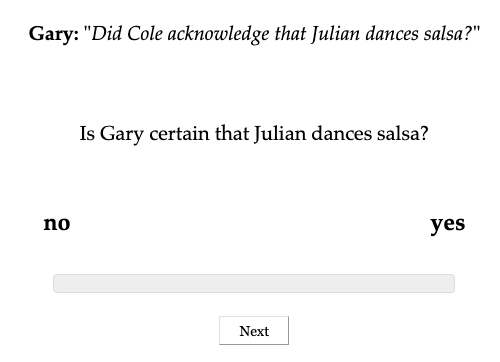
\includegraphics[height=4.4cm,width=7.6cm]{figures/2q-proj}}
\caption{Exps.~1q, 2q, and 3q.}\label{fig-exp1q-projection}
\end{subfigure}%
\begin{subfigure}[t]{0.5\textwidth}
\centering
\fbox{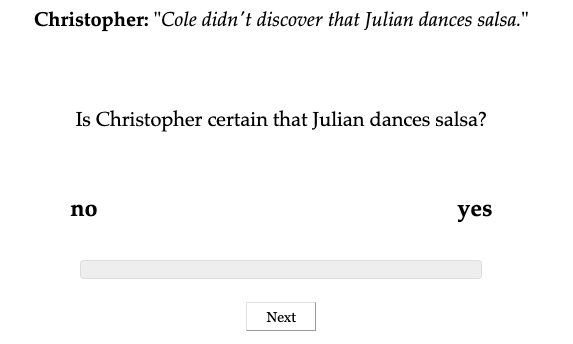
\includegraphics[height=4.4cm,width=7.6cm]{figures/1n-proj}} 
\caption{Exps.~1n, 2n, and 3n.}\label{fig-exp1n-projection}
 \end{subfigure}
\begin{subfigure}[t]{0.5\textwidth}
        \centering
\fbox{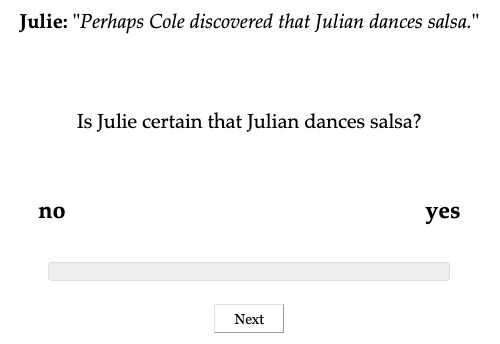
\includegraphics[height=4.4cm,width=7.6cm]{figures/1m-proj}}
\caption{Exps.~1m, 2m, and 3m}\label{fig-exp1m-projection}
 \end{subfigure}%
\begin{subfigure}[t]{0.5\textwidth}
\centering
\fbox{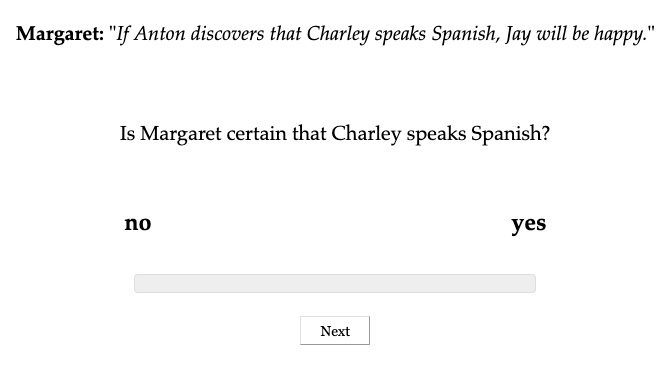
\includegraphics[height=4.4cm,width=7.6cm]{figures/1c-proj}} 
\caption{Exps.~1c, 2c, and 3c}\label{fig-exp1c-projection}
\end{subfigure}
\caption{Target trials in projection blocks of Exps.~1, 2, and 3 for the complement {\em Julian dances salsa}.}\label{fig:projection-trials}
\end{figure}

In the at-issueness blocks of Exps.~1-3, the 20 clauses were also realized as the complements of the 20 clause-embedding predicates in Fig.~\ref{fig:predicates} and the target stimuli realized either a polar question sentence (in Exps.~1q, 2q, and 3q), a negated sentence (in Exps.~1n, 2n, and 3n), a sentence with {\em perhaps} (in Exps.~1m, 2m, 3m), or a conditional sentence (in Exps.~1c, 2c, 3c). Sample trials of the at-issueness measures implemented in the 12 experiments are provided in Fig.~\ref{fig:ai-exps1} for Exps.~1, in Fig.~\ref{fig:ai-exps2} for Exps.~2, and in Fig.~\ref{fig:ai-exps3} for Exps.~3. Across all these measures, participants gave their responses on a slider marked `no' at one end (coded as 1) and `yes' at the other (coded as 0). Greater not-at-issueness of the CC should result in higher slider ratings.

\begin{figure}[h!]
\centering

\begin{subfigure}[t]{0.5\textwidth}
        \centering
\fbox{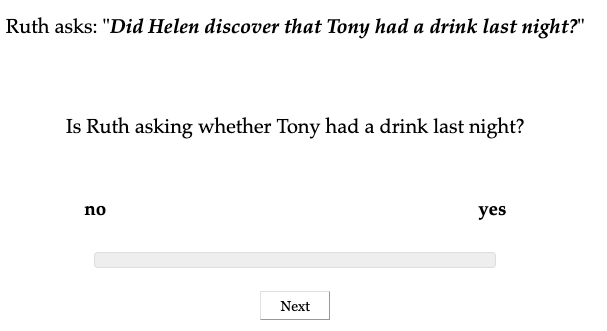
\includegraphics[height=5.4cm,width=7.6cm]{figures/1q-ai}}
\caption{Exp.~1q.}
\end{subfigure}%
\begin{subfigure}[t]{0.5\textwidth}
\centering
\fbox{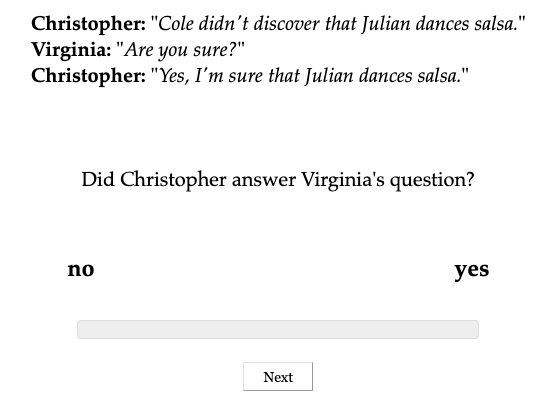
\includegraphics[height=5.4cm,width=7.6cm]{figures/1n-ai}} 
\caption{Exp.~1n.}
 \end{subfigure}
\begin{subfigure}[t]{0.5\textwidth}
        \centering
\fbox{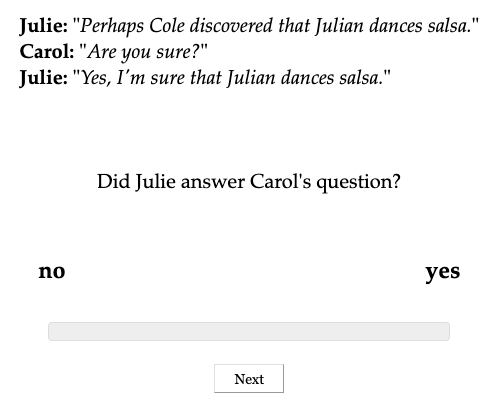
\includegraphics[height=5.4cm,width=7.6cm]{figures/1m-ai}}
\caption{Exp.~1m}
 \end{subfigure}%
 \begin{subfigure}[t]{0.5\textwidth}
        \centering
\fbox{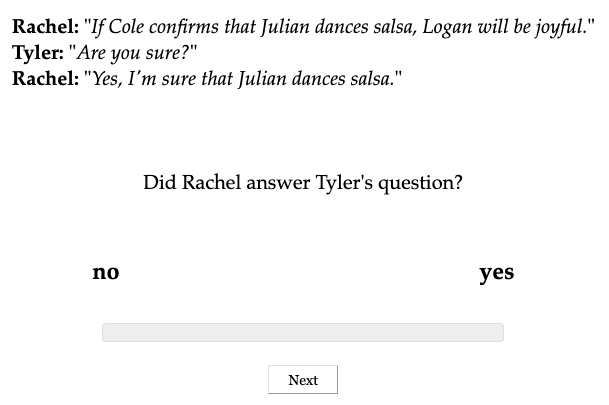
\includegraphics[height=5.4cm,width=7.6cm]{figures/1c-ai}}
\caption{Exp.~1c}
 \end{subfigure}

\caption{Target trials in at-issueness blocks of Exps.~1 for the complement {\em Julian dances salsa}.}\label{fig:ai-exps1}
\end{figure}

\begin{figure}[h!]
\centering

\begin{subfigure}[t]{0.5\textwidth}
        \centering
\fbox{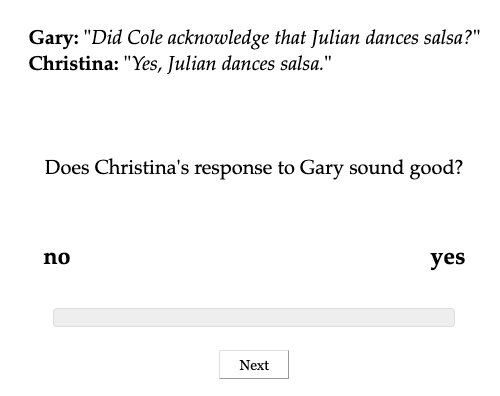
\includegraphics[height=5.4cm,width=7.6cm]{figures/2q-ai}}
\caption{Exp.~2q.}
\end{subfigure}%
\begin{subfigure}[t]{0.5\textwidth}
\centering
\fbox{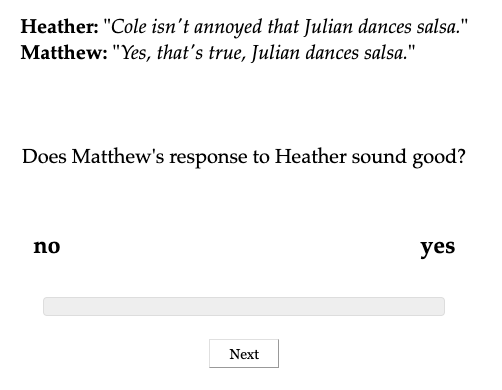
\includegraphics[height=5.4cm,width=7.6cm]{figures/2n-ai}} 
\caption{Exp.~2n.}
 \end{subfigure}
\begin{subfigure}[t]{0.5\textwidth}
        \centering
\fbox{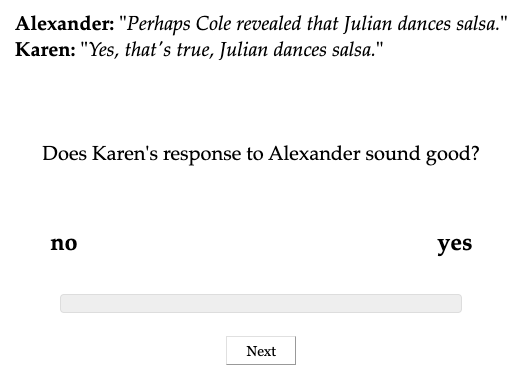
\includegraphics[height=5.4cm,width=7.6cm]{figures/2m-ai}}
\caption{Exp.~2m}
 \end{subfigure}%
 \begin{subfigure}[t]{0.5\textwidth}
        \centering
\fbox{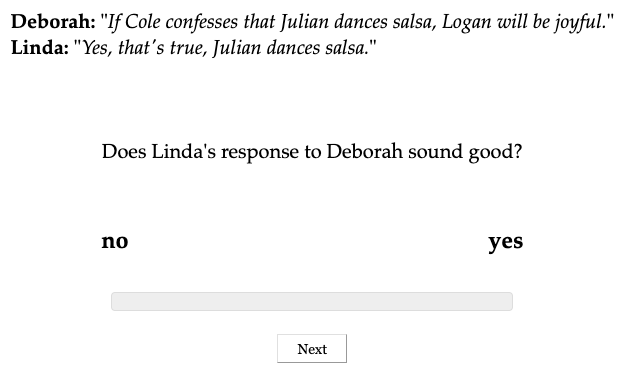
\includegraphics[height=5.4cm,width=7.6cm]{figures/2c-ai}}
\caption{Exp.~2c}
 \end{subfigure}

\caption{Target trials in at-issueness blocks of Exps.~2 for the complement {\em Julian dances salsa}.}\label{fig:ai-exps2}
\end{figure}

\begin{figure}[h!]
\centering

\begin{subfigure}[t]{0.5\textwidth}
        \centering
\fbox{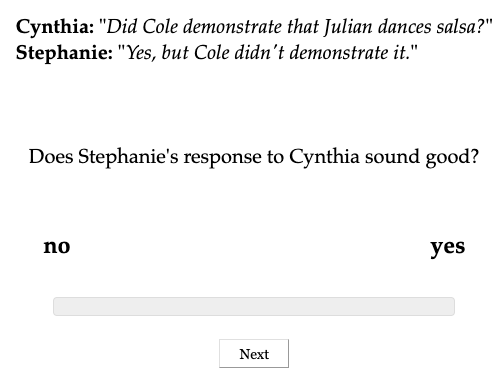
\includegraphics[height=5.4cm,width=7.6cm]{figures/3q-ai}}
\caption{Exp.~3q.}
\end{subfigure}%
\begin{subfigure}[t]{0.5\textwidth}
\centering
\fbox{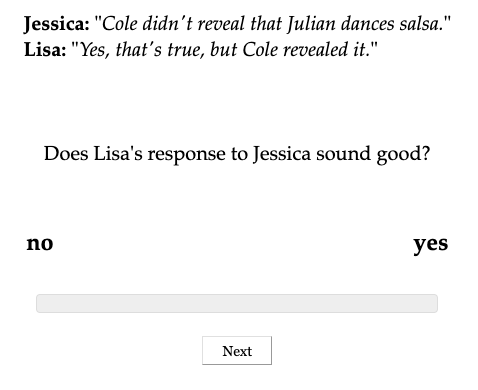
\includegraphics[height=5.4cm,width=7.6cm]{figures/3n-ai}} 
\caption{Exp.~3n.}
 \end{subfigure}
\begin{subfigure}[t]{0.5\textwidth}
        \centering
\fbox{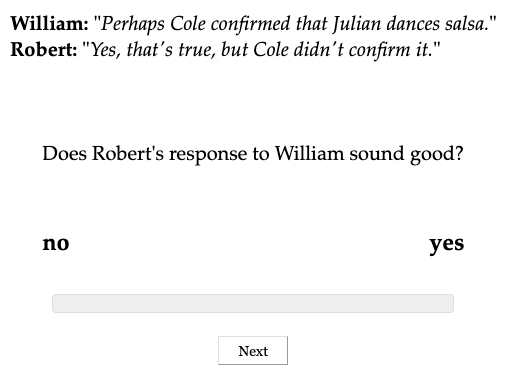
\includegraphics[height=5.4cm,width=7.6cm]{figures/3m-ai}}
\caption{Exp.~3m}
 \end{subfigure}%
 \begin{subfigure}[t]{0.5\textwidth}
        \centering
\fbox{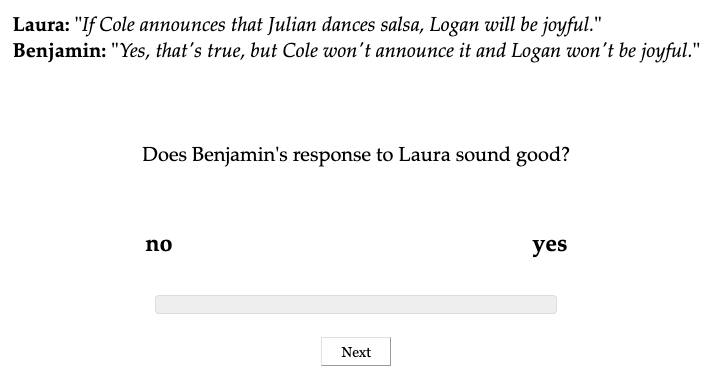
\includegraphics[height=5.4cm,width=7.6cm]{figures/3c-ai}}
\caption{Exp.~3c}
 \end{subfigure}

\caption{Target trials in at-issueness blocks of Exps.~3 for the complement {\em Julian dances salsa}.}\label{fig:ai-exps3}
\end{figure}


To assess whether participants were attending to the task, each experiment also included six control stimuli, which were also utterances made by a named speaker. Depending on the experiment, the content of these stimuli was expected to receive either high or low certainty ratings, and either high or low ratings on the at-issueness measure; see Supplement \ref{a-control} for details and the control stimuli.

Participants were told to imagine that they are at a party and that, on walking into the kitchen, they overhear somebody say something to somebody else. Each participant saw a random set of 26 stimuli: each set contained one target utterance for each of the 20 contents (each paired with a unique clause-embedding predicates) and the same 6 (experiment-specific) control stimuli. Each participant saw their set of 26 stimuli twice, once in the projection block and once in the at-issueness block. Block order and within-block trial order was randomized. After completing the experiment, participants filled out a short optional demographic survey. To encourage truthful responses, participants were told that they would be paid no matter what answers they gave in the survey.

\subsection{Data exclusion} 

We excluded data from participants who took any experiment more than once and who did not self-declare to be native speakers of American English. We also excluded data from participants based on their ratings on the main clause controls and other criteria given in Supplement \ref{a-participants}. In each experiment, the data from between 215-281 remaining participants were analyzed. Information on the participants whose data entered into the analysis (total number, ages, gender) can be found in Supplement \ref{a-participants}.

\newpage

\section{Projection}

Compare projectivity ratings across entailment-cancelling operators. 
\begin{itemize}
  \item is there a difference between projectivity across contexts? 
  \item is there a difference between verbs in terms of how much embedding context makes a difference (semi-factive v factive)?
  \item previous point that non-factive (i.e. veridical) predicates can also project can be made here for other embedding operators as well
\end{itemize}

\section{At-issueness}

At-issueness diagnostics (kind of) work for questions:
\begin{itemize}
  \item asking whether diagnostic (exp. 1q)
  \item Q-A diagnostic (exp. 2q)
\end{itemize}


\section{GPP}

Replicating results from \cite{tbd-variability}: Correlation between NAI \& projection for PolQs found for:
\begin{itemize}
  \item asking whether diagnostic (exp. 1q)
  \item Q-A diagnostic (exp. 2q)
\end{itemize}

\noindent Both of these also show some interesting lexical exceptions:
\begin{itemize}
  \item non-veridical predicates
  \item some specific kinds of reportatives
  \item how can we systematically identify exceptions based on data analysis?
  \item are these the same kinds of exceptions as in the glossa paper?
\end{itemize}


\noindent Further analyses:
\begin{itemize}
  \item look at how many unique participants

  \item negative correlation between Q/A and assent might be compound of a) embedding (negation) and b) assent, because we don?t see negative correlation, but no correlation, with other embeddings (modal, conditional)

  \item  compare variance for both projection and at-issueness, under the different embeddings and diagnostics: very little variance for assent diagnostic/negation embedding

  \item have a look at the predicates that are exceptional to the GPP in Exps1 and 2, how do they behave across the other experiments? Exp3: looks like they are also their own little group

  \item  when we compare negation, modal, conditional with assent diagnostic, we can see what effect embedding has

  \item next experiments: no embedding of the 20 predicates, with assent diagnostic, to compare to prior literature who didn?t use embedding with the assent diagnostic; do assent diagnostic without ?that?s true? anaphor to engage with Snider?s assumption that ?yes? is not really anaphoric in the assent diagnostic and hence also not in the Q/A diagnostic

\end{itemize}

\section{General discussion}\label{s4}

\section{Conclusions}\label{s5}

% end document here for word count
%\end{document}

\bibliographystyle{cslipubs-natbib}
\bibliography{bibliography}

\newpage

\section*{Supplemental materials}

\appendix

\setcounter{page}{1}
%\renewcommand{\thetable}{A\arabic{table}}

\setcounter{table}{0}
\renewcommand{\thetable}{A\arabic{table}}

\setcounter{figure}{0}
\renewcommand{\thefigure}{A\arabic{figure}}

\section{20 clauses}\label{a-clauses}

The contents of the following 20 clauses, which realized the complements of the 20 clause-embedding predicates, were investigated in Exps.~1-3:

\begin{enumerate}[leftmargin=3ex,itemsep=-2pt]

\begin{multicols}{2}

\item Mary is pregnant.
\item Josie went on vacation to France.
\item Emma studied on Saturday morning.
\item Olivia sleeps until noon.
\item Sophia got a tattoo.
\item Mia drank 2 cocktails last night.
\item Isabella ate a steak on Sunday.
\item  Emily bought a car yesterday.
\item  Grace visited her sister.
\item Zoe calculated the tip.

\columnbreak

\item  Danny ate the last cupcake.
\item  Frank got a cat.
\item  Jackson ran 10 miles.
\item  Jayden rented a car.
\item  Tony had a drink last night.
\item  Josh learned to ride a bike yesterday.
\item  Owen shoveled snow last winter.
\item  Julian dances salsa.
\item  Jon walks to work.
\item  Charley speaks Spanish.

\end{multicols}

\end{enumerate}

\section{Consequents for conditional target stimuli in Exps.~1c, 2c, and 3c}\label{a-consequents}

We created 20 consequent clauses for the three experiments in which the 20 clauses were embedded in the antecedent of a conditional (Exps.~1c, 2c, 3c). Each of the 20 clauses was paired with a unique consequent clause, as shown in the list below. To minimize the variability of the effect of the contents of these consequent clauses on the projection of the contents of the 20 complement clauses, the consequent clauses all consist of a uniquely named subject and an adjectival predication in the future tense ({\em will be}), and the adjectives all denote an emotion. We selected the 20 emotion-denoting adjectives based on the valence and arousal values reported in \citealt{warriner-etal2013}: 10 of the adjectives had a positive valence, and 10 had a negative valence; all 20 adjective had an arousal value between 4.7 and 6.5. 

\begin{enumerate}[leftmargin=3ex,itemsep=-2pt]

\item \ldots that Mary is pregnant, Esther will be mad.
\item \ldots that Josie went on vacation to France, Arnold will be frustrated.
\item \ldots that Emma studied on Saturday morning, Liam will be proud.
\item \ldots that Olivia sleeps until noon, Elijah will be embarrassed.
\item \ldots that Sophia got a tattoo, Ariel will be giddy.
\item \ldots that Mia drank 2 cocktails last night, Mariela will be worried.
\item \ldots that Isabella ate a steak on Sunday, Liz will be delighted.
\item  \ldots that Emily bought a car yesterday, Kate will be excited.
\item \ldots that  Grace visited her sister, Henry will be surprised.
\item \ldots that Zoe calculated the tip, Alex will be astonished.
\item  \ldots that Danny ate the last cupcake, Harper will be disgusted.
\item  \ldots that Frank got a cat, Lucas will be grouchy.
\item  \ldots that Jackson ran 10 miles, Kayla will be cheerful.
\item  \ldots that Jayden rented a car, Brittany will be furious.
\item  \ldots that Tony had a drink last night, Victoria will be ashamed.
\item  \ldots that Josh learned to ride a bike yesterday, Mason will be envious.
\item  \ldots that Owen shoveled snow last winter, Bianca will be jealous.
\item  \ldots that Julian dances salsa, Logan will be joyful.
\item  \ldots that Jon walks to work, Caleb will be suspicious.
\item  \ldots that Charley speaks Spanish, Jay will be happy.

\end{enumerate}

\section{Control stimuli in Exps.~1-3}\label{a-control}

The control stimuli in Exps.~1-3 were the contents of main clauses. In Exps.~1q, 2q and 3q, the control stimuli consisted of the polar questions in (1). The non-restrictive relative clauses (NRRCs), given in parentheses in (1), were included in Exps.~2q and 3q, where at-issueness was measured with an assent diagnostic. The control stimuli here consisted of two clauses (like the target stimuli), to allow the relevant speaker to assent with one of two clauses.

\begin{exe}
\exi{(1)} Sentences for control stimuli in in question embedding experiments (Exps.~1q, 2q and 3q)
\begin{xlist}
\ex Do these muffins (, which are really delicious,) have blueberries in them?
\ex Does this pizza (, which I just made from scratch,) have mushrooms on it? 
\ex Was Jack (, who is my long-time neighbor,) playing outside with the kids? 
\ex Does Ann (, who is a local performer,) dance ballet?
\ex Were John's kids (, who are very well-behaved,) in the garage?
\ex Does Samantha (, who is really into fashion,) have a new hat?
\end{xlist}
\end{exe}

We expected participants to give low responses on the `certain that' diagnostic for the control stimuli in (1), indicating that the speaker is not certain of the main clause content, because main clause content is hypothesized to not project out of polar questions. These expectations were borne out, as shown in the third column of Table~\ref{t-controls} for Exps.~1q, 2q, and 3q. We also expected participants to give low responses on the at-issueness diagnostics for the control stimuli in (1), indicating that the main clause content is at-issue. These expectations were borne out for Exps.~1q and 2q, as shown in the fourth column of Table~\ref{t-controls}, but the ratings were higher than expected for Exp.~3q. See below for discussion.


In the remaining experiments, the control stimuli consisted of the positive declarative variants of (1) given in (2). The NRRCs in parentheses were realized in Exps.~2 and 3 for the reason explained above, as well as in Exp.~1c, to make the control stimuli more similar to the target stimuli (which also consisted of two clauses, namely the antecedent and the consequent).

\begin{exe}
\exi{(2)}  Sentences for control stimuli in negation, modal and conditional embeddings
\begin{xlist}
\ex These muffins (, which are really delicious,) have blueberries in them.
\ex This pizza (, which I just made from scratch,) has mushrooms on it. 
\ex Jack (, who is my long-time neighbor,) was playing outside with the kids. 
\ex Ann (, who is a local performer,) dances ballet.
\ex John's kids (, who are very well-behaved,) were in the garage.
\ex Samantha (, who is really into fashion,) has a new hat.
\end{xlist}
\end{exe}

We expected participants to give high responses on the `certain that' diagnostic for the control stimuli in (2), indicating that the speaker is certain of the main clause content, because speakers are hypothesized to be committed to the asserted main clause content. These expectations were borne out, as shown in the third column of Table~\ref{t-controls} for the `n', `m' and `c' variants of Exps.~1, 2, and 3. We expected participants to give low responses on the at-issueness diagnostics for the control stimuli in (2), indicating that the main clause content is at-issue. These expectations were borne out for the `n', `m', and `c' variants of Exps.~1, as shown in the fourth column of Table~\ref{t-controls}, but not for the `n', `m', and `c' variants of Exps.~2 and 3. See below for discussion.

\begin{table}[h!]
\centering
\begin{tabular}{r r r r l }
& &  \multicolumn{2}{c}{Mean ratings} &  \\ 
Exp. & Control stimuli & Certainty & Not-at-issueness & At-issueness measure \\ 
\hline
1q & (1) & .14 & .05  & asking whether $c$ \\
1n & (2) &  .95 & .04 & sure that $c$\\
1m & (2) & .96 & .03 & sure that $c$\\
1c & (2) with NRRC & .94  & .08 & sure that $c$\\
\hline
2q & (1) with NRRC & .18 & .07 & {\em yes}, $c$\\
2n & (2) with NRRC& .96 & .22 & {\em yes, that's true}, $c$\\
2m & (2) with NRRC& .96 & .25 & {\em yes, that's true}, $c$\\
2c & (2) with NRRC& .96 & .22 & {\em yes, that's true}, $c$\\
\hline
3q & (1) with NRRC & .17 &  .28 & {\em yes}, but $\neg c'$\\
3n & (2) with NRRC & .94 & .44 & {\em yes, that's true}, but $\neg c'$\\
3m & (2) with NRRC & .93 & .50 & {\em yes, that's true}, but $\neg c'$\\
3c & (2) with NRRC & .93 & .53 & {\em yes, that's true}, but $\neg c'$\\
\hline
\end{tabular}
\caption{Mean certainty and at-issueness ratings for control stimuli, for self-declared American English participants}\label{t-controls}
\end{table}

As mentioned above, the mean at-issueness ratings were higher than expected in the `n', `m', and `c' variants of Exps.~2 and all four of the Exps.~3. We discuss these exceptions in more detail here because they allow us to further understand the various measures for at-issueness investigated in this paper. The example in (3a) illustrates the version of the assent diagnostic applied in Exps.~2n, 2m, and 2c: the assent particle {\em yes} is followed by the clause whose content is diagnosed, here, the content of the main clause. The related affirmation diagnostic applied in Exp.~2q (where the mean at-issueness rating was as low as expected) is illustrated in (3b).

\begin{exe}
\exi{(3)} 
\begin{xlist}
\ex Sample control stimulus in Exps.~2n, 2m, and 2c
\begin{xlist}
\exi{A:} These muffins, which are really delicious, have blueberries in them.
\exi{B:} Yes, that's true, they have blueberries in them.
\end{xlist}
Question to participants: Does A's response to B sound good?
\ex Sample control stimulus in Exp.~2q
\begin{xlist}
\exi{A:} Do these muffins, which are really delicious, have blueberries in them?
\exi{B:} Yes, they have blueberries in them.
\end{xlist}
Question to participants: Does A's response to B sound good?
\end{xlist}
\end{exe}
As shown in Table \ref{t-controls},  the group mean on the control stimuli is numerically higher (at .22 or .25) than for Exp.~2q (.07). We hypothesize that a possible explanation for this difference is that participants take A to assert both the content of the main clause and of the NRRC in (3a) but is only asking about the main clause content in (3b). Whereas B's affirmation in (3b) specifies the one content that is affirmed, B's assent in (3a) specifies only one of the two contents that A asserted, seemingly leaving out a specification of the second content, that of the NRRC. Participants may judge B's response in (3b) to be less acceptable than in (3a) because of this missing content specification. This hypothesis is consistent with the results of \citepos{syrett-koev2015} Exp.~3, which suggests that content of a sentence-medial NRRCs can be the target of a direct denial, though the main clause content is preferred as the target of such a denial. That the group means on the control stimuli in our Exps.~2n, 2m, and 2c are still relatively low may be due to the fact that the one content that was specified is the at-issue main clause content. One would expect lower acceptability ratings in a version of this diagnostic in which the one content that was specified is the NRRC. 

The mean at-issueness ratings for the control stimuli were also higher than expected in Exps.~3. The examples in (4) illustrate the versions of the affirmation and assent diagnostics used in these experiments:

\begin{exe}
\exi{(4)} 
\begin{xlist}
\ex Sample control stimulus in Exp.~3q
\begin{xlist}
\exi{A:} Do these muffins, which are really delicious, have blueberries in them?
\exi{B:} Yes, but they aren't really delicious.
\end{xlist}
Question to participants: Does A's response to B sound good?
\ex Sample control stimulus in Exps.~3n, 3m, and 3c
\begin{xlist}
\exi{A:} These muffins, which are really delicious, have blueberries in them.
\exi{B:} Yes, that's true, they but they aren't really delicious.
\end{xlist}
Question to participants: Does A's response to B sound good?
\end{xlist}
\end{exe}
The mean at-issueness rating for the control stimuli in Exp.~3q was comparatively higher (at .28) than for Exp.~1q (.05) or Exp.~2q (.07). We hypothesize that that this difference (especially to Exp.~2q) is due the content of the NRRC being directly denied, even though it was presented as backgrounded content in A's question (as shown in (2), the content of none of the other NRRCs was a matter of personal taste).

The mean at-issueness ratings for the control stimuli in Exps.~3n, 3m, and 3c were numerically even higher than for Exp.~3q and, in fact, the highest across all 12 experiments (at .44, .50, and .53, respectively). There are two factors that could be implicated in the difference between Exp.~3q and Exps.~3n, 3m, and 3c: first, the NRRC is included in a polar question in the former but a declarative assertion in the latter; second, B utters an affirmation {\em yes} in the former but an assent {\em yes, that's true} in the latter. For instance, participants might judge B's direct denial of the content of the NRRC as less acceptable when A uttered a declarative assertion and B assented with that assertion using {\em yes, that's true} than when A uttered a polar question and B responded in the affirmative with {\em yes}. Both factors must be considered in future research on at-issueness measures.


\section{Participant information and data exclusion criteria}\label{a-participants}

This supplement provides information on the participants of the 12 experiments and the criteria by which participants' data were excluded. The first three columns of Table \ref{t:exclusion} show, for each of the 12 experiments how many participants were recruited, their age range and mean age, and their self-reported gender; no gender data was collected in Exp.~1q. The next three columns provide information on the number of participants whose data were excluded based on the following criteria:

\begin{itemize}[itemsep=-2pt]

\item `multiple': Due to an experimental glitch, some participants participated more than once in Exp.~1q. Since no information was available on which one was their first take, those participants' data was removed. 

\item `language': Participants' data were excluded if they did not self-identify as native speakers of American English.

\item `controls': Participants' data were excluded if their mean rating on the 6 main clause control items in the projection block was more than 2 sd above the group mean (in Exps.~1q, 2q, and 3q) or more than 2 sd below the group mean (in the remaining experiments). Participants' data were also excluded if their mean rating on the 6 main clause control items in the at-issueness block was more than 2 sd above the group mean (across all experiments).
 
\item `variance': Participants' data were excluded if they always selected roughly the same point on the response scale for the target stimuli. To identify such participants, we first identified participants whose mean variance on the target stimuli was more than 2 sd below the group mean variance and then manually inspecting their response patterns. The data of participants who used the full scale was not excluded.  
\end{itemize}

The remaining columns of Table \ref{t:exclusion} provide information on the remaining participants, that is, the participants' data that entered into the analysis. Participants took around 9-11 minutes to complete the various experiments. Participants were paid more in Exps.~1c, 2c, and 3c than the remaining experiments because the target stimuli in those experiments were longer (as they consisted of conditionals). More women than men were recruited in many of the experiments because the experiments were run at a time when Prolific went viral on TikTok, resulting in a large number of young women registering for the service (around July 24, 2021; see \url{https://blog.prolific.co/we-recently-went-viral-on-tiktok-heres-what-we-learned/}, \\ last accessed February 4, 2022).  

\begin{sidewaystable}[h!]
\centering
\begin{tabular}{l | r r r | r r r r | r r r | r }
&  \multicolumn{3}{c|}{Recruited participants} & \multicolumn{4}{c|}{Exclusion criteria} & \multicolumn{3}{c|}{Remaining participants} &  \\ 
Exp. & total & ages (mean) & gender (f/m/o/u) & multiple & language & controls & variance & total & ages (mean) & gender (f/m/o/u) & payment   \\ 
\hline
1q & 300  & 19-74 (38.2)  & --  & 5  & 7  & 35  & 0  & 242   & 21-74 (39.2) &  -- & \$1.70\\
1n & 300  & 18-74 (33.2)  &  150/145/5/0 & 0  & 8 & 17 & 1 & 274  & 18-74 (33.3) & 141/128/5/0 & \$1.70\\
1m & 300  & 18-74 (32.7) & 150/141/7/2  &  0 & 0  & 19 & 0   & 281   & 18-74 (32.7) & 144/129/7/1 & \$1.70 \\
1c &  300 & 18-58 (25.9)  & 249/45/6/0 & 0 & 6  & 26 & 2  & 266  &  18-58 (24.8) & 235/25/6/0  & \$2.15 \\
2q & 250  &  18-58 (25.5) &  201/43/6/0  & 0 & 4  & 24  & 1 & 220  & 18-58 (24.8)  & 187/28/5/0  & \$1.70 \\
2n & 250  &  18-69 (33.2)  &  127/114/6/1 & 1  & 4  & 29 & 0& 215  &  18-69 (33.1) & 113/95/6/1    & \$1.70\\
2m & 251  & 18-74 (31.7)  & 132/113/6/0  & 0  & 4  & 27 &  0 & 220  & 18-70 (31.9) & 116/98/6/0 & \$1.70\\
2c &  250 &  18-56 (24.5)  & 212/30/8/0  & 0  & 0  & 26 & 0  & 224  & 18-56 (24.4) & 195/24/5/0 & \$2.15\\
3q & 250  &  18-66 (32.4) &  140/102/7/1 &  0 & 4  & 20  & 0  &  225 & 18-66 (32.6) & 125/93//7/0  & \$1.70 \\
3n & 250  &  18-70 (24.6) & 114/31/5/0  & 0  & 5  &  13 & 4  & 228  & 18-70 (24.3) &  198/25/5/0 &\$1.70 \\
3m & 250  & 18-63 (25.5)  & 205/40/5/0 &  0 & 3  & 14 &  0 & 233  &  18-63 (24.8) & 197/31/5/0 &\$1.70 \\
3c & 250  & 18-59  (27.5) & 182/64/4/0  & 0  & 3  & 17 & 0 & 230  &  18-59 (26.7)  & 177/49/4/0  & \$2.15\\
\end{tabular}
\caption{Recruited participants, excluded data, and remaining participants in Exps.~1, 2 and 3. Gender distinctions were `f' = female, `m' = male, `o' = other, and `u' = undeclared.}\label{t:exclusion}
\end{sidewaystable} 
 
\end{document}

